%%%%%%%%%%%%%%%%%%%%%%%%%%%%%%%%%%%%%%%%%
% Masters/Doctoral Thesis 
% LaTeX Template
% Version 1.42 (19/1/14)
%
% This template has been downloaded from:
% http://www.latextemplates.com
%
% Original authors:
% Steven Gunn 
% http://users.ecs.soton.ac.uk/srg/softwaretools/document/templates/
% and
% Sunil Patel
% http://www.sunilpatel.co.uk/thesis-template/
%
% License:
% CC BY-NC-SA 3.0 (http://creativecommons.org/licenses/by-nc-sa/3.0/)
%
% Note:
% Make sure to edit document variables in the Thesis.cls file
%
%%%%%%%%%%%%%%%%%%%%%%%%%%%%%%%%%%%%%%%%%

%----------------------------------------------------------------------------------------
%	PACKAGES AND OTHER DOCUMENT CONFIGURATIONS
%----------------------------------------------------------------------------------------

\documentclass[11pt, a4paper, oneside]{Thesis} % Paper size, default font size and one-sided paper
\graphicspath{{./Pics/}}
\usepackage[square, numbers, comma, sort&compress]{natbib} % Use the natbib reference package - read up on this to edit the reference style; if you want text (e.g. Smith et al., 2012) for the in-text references (instead of numbers), remove 'numbers' 
\usepackage{url}
\usepackage{listings}
\usepackage{amsmath}
\usepackage[ngerman]{babel}
\hypersetup{urlcolor=blue, colorlinks=true} % Colors hyperlinks in blue - change to black if annoying
\title{\ttitle} % Defines the thesis title - don't touch this

\begin{document}
\lstset{language=Java,
		mathescape}
\frontmatter % Use roman page numbering style (i, ii, iii, iv...) for the pre-content pages

\setstretch{1.3} % Line spacing of 1.3

% Define the page headers using the FancyHdr package and set up for one-sided printing
\fancyhead{} % Clears all page headers and footers
\rhead{\thepage} % Sets the right side header to show the page number
\lhead{} % Clears the left side page header

\pagestyle{fancy} % Finally, use the "fancy" page style to implement the FancyHdr headers

\newcommand{\HRule}{\rule{\linewidth}{0.5mm}} % New command to make the lines in the title page

% PDF meta-data
\hypersetup{pdftitle={\ttitle}}
\hypersetup{pdfsubject=\subjectname}
\hypersetup{pdfauthor=\authornames}
\hypersetup{pdfkeywords=\keywordnames}

%----------------------------------------------------------------------------------------
%	TITLE PAGE
%----------------------------------------------------------------------------------------

\begin{titlepage}
\begin{center}

\textsc{\LARGE \univname}\\[1.5cm] % University name
\textsc{\Large Bachelorarbeit}\\[0.5cm] % Thesis type

\HRule \\[0.4cm] % Horizontal line
{\huge \bfseries \ttitle}\\[0.4cm] % Thesis title
\HRule \\[1.5cm] % Horizontal line
 
\begin{minipage}{0.4\textwidth}
\begin{flushleft} \large
\emph{Author:}\\
\authornames % Author name - remove the \href bracket to remove the link
\end{flushleft}
\end{minipage}
\begin{minipage}{0.4\textwidth}
\begin{flushright} \large
\emph{Supervisor:} \\
\supname% Supervisor name - remove the \href bracket to remove the link  
\end{flushright}
\end{minipage}\\[3cm]
 
\large \textit{A thesis submitted in fulfilment of the requirements\\ for the degree of \degreename}\\[0.3cm] % University requirement text
\textit{in the}\\[0.4cm]
\groupname\\\deptname\\[2cm] % Research group name and department name
 
{\large \today}\\[4cm] % Date
%\includegraphics{Logo} % University/department logo - uncomment to place it
 
\vfill
\end{center}

\end{titlepage}

%----------------------------------------------------------------------------------------
%	DECLARATION PAGE
%	Your institution may give you a different text to place here
%----------------------------------------------------------------------------------------

\Declaration{

\addtocontents{toc}{\vspace{1em}} % Add a gap in the Contents, for aesthetics

Ich, \authornames, best\"atige hiermit, dass die Bachelorarbeit mit dem Titel '\ttitle' und das dazugeh\"orige Programm selbstst\"andig von mir geschrieben wurde. Ich best\"atige:

\begin{itemize} 
\item[\tiny{$\blacksquare$}] Diese Arbeit wurde komplett w\"ahrend meiner Studienzeit an der Universtit\"at Bielefeld f\"ur den Bachelor of Science geschrieben.
\item[\tiny{$\blacksquare$}] Ich habe die einbezogene Arbeit von anderen immer deutlich kenntlich gemacht.
\item[\tiny{$\blacksquare$}] Ich habe zu jedem Zitat die Quelle angeben. Au\ss erhalb dieser Zitate habe ich alles selbst\"antig verfasst.

\end{itemize}
\vspace*{-\baselineskip}
\vspace{4cm}
Signed:\\
\rule[1em]{25em}{0.5pt} % This prints a line for the signature
 
Date:\\
\rule[1em]{25em}{0.5pt} % This prints a line to write the date
}

\clearpage % Start a new page

%----------------------------------------------------------------------------------------
%	ABBREVIATIONS
%----------------------------------------------------------------------------------------

\setstretch{1.5} % Set the line spacing to 1.5, this makes the following tables easier to read

\lhead{\emph{Abk\"urzungen}} % Set the left side page header to "Abbreviations"
\listofsymbols{ll} % Include a list of Abbreviations (a table of two columns)
{
\textbf{ERU} & \textbf{E}ntity-\textbf{R}ecognition-\textbf{U}nit \\
\textbf{GUI} & \textbf{G}raphical \textbf{U}ser \textbf{I}nterface \\
\textbf{IBEL} & \textbf{I}ndex \textbf {B}ased \textbf{E}ntity \textbf{L}inker \\
\textbf{IBELU} & \textbf{I}ndex \textbf {B}ased \textbf{E}ntity \textbf{L}inker \textbf{U}tility \\
\textbf{idf} & \textbf{i}nverse \textbf{d}ocument \textbf{f}requency \\
\textbf{JAR} & \textbf{J}ava \textbf{AR}chieve \\
\textbf{NER} & \textbf{N}amed \textbf{E}ntity \textbf{R}ecognizer \\
\textbf{RDF} & \textbf{R}esource \textbf{D}escription \textbf{F}ramework \\
\textbf{tf} & \textbf{t}erm \textbf{f}requency \\
\textbf{URI} & \textbf{U}niform \textbf{R}esource \textbf{I}dentifier \\
%\textbf{} & \textbf{} \textbf{} \textbf{} \\
%\textbf{Acronym} & \textbf{W}hat (it) \textbf{S}tands \textbf{F}or \\
}
\pagestyle{fancy} % The page style headers have been "empty" all this time, now use the "fancy" headers as defined before to bring them back

%----------------------------------------------------------------------------------------
%	LIST OF CONTENTS/FIGURES/TABLES PAGES
%----------------------------------------------------------------------------------------

\clearpage
\lhead{\emph{Abbildungsverzeichnis}} % Set the left side page header to "List of Figures"
\listoffigures % Write out the List of Figures
%\lhead{\emph{Contents}} % Set the left side page header to "Contents"
\tableofcontents % Write out the Table of Contents




%----------------------------------------------------------------------------------------
%	THESIS CONTENT - CHAPTERS
%----------------------------------------------------------------------------------------

\mainmatter % Begin numeric (1,2,3...) page numbering

\pagestyle{fancy} % Return the page headers back to the "fancy" style

% Include the chapters of the thesis as separate files from the Chapters folder
% Uncomment the lines as you write the chapters
\chapter{Einleitung}
\label{Kapitel 1}

\lhead{Kapitel 1.}
\chead{\emph{Einleitung}}
In der heutigen Zeit spielen Wissensdatenbanken wie Wikipedia\footnote{\url{wikipedia.org}} eine immer gr\"o\ss ere Rolle. Sie repr\"asentieren das gesammelte Wissen der Menschheit und stellen es zur freien Verf\"ugung. Eine wichtige Eigenschaft von Wikipedia ist die Reichhaltigkeit von eingebetteten Links in jedem Artikel, welche die wichtigsten Terme mit anderen Seiten verknüpfen und somit einem Benutzer einen schnellen Weg zu zus\"aztlichen Informationen zu gew\"ahren\citep{rada07}.\\
W\"ahrend diese Links in Wikipedia, dank der massiven Anzahl an Beitragenden, manuell erstellt werden k\"onnen, ist f\"ur viele andere Dienste, wie zum Beispiel Web-Personensuche und Informationsextraktion, eine automatisierte L\"osung gew\"unscht. Die daf\"ur n\"otige Named-Entity-Disambiguierung ist problematisch, da eine Entit\"at multiple Benennungen hat und diese unter Umst\"anden auch mit anderen Entit\"aten teilt \cite{wei10}.\\
Die Aufgabe des Entity-Linkings ist es, Entit\"aten aus einem Webtext mit dem \"Aquivalent aus einer Wissensdatenbank zu verbinden. Dies ist nicht zu verwechseln mit dem named entity recognition Prozess, der sich auf die Identifizierung von Dingen in einem Text und nicht auf die Suche nach der Referenz, die diese Entit\"at darstellt beschr\"ankt. Eine solche Disambiguierung kann zum Beispiel, wie in dieser Arbeit und \citep{mil08} vorstellt, mit der Hilfe von Anchors erfolgen.


\section{Verwandte Arbeiten}
\subsection{DBpedia}
%\footnote{\url{dbpedia.org}}
W\"ahrend die meisten Wissensdatenbanken heutzutage auf spezifische Dom\"anen beschr\"ankt sind und von einer kleinen Gruppe von Wissensmodelierern, unter hohen Kosten, erstellt und gewartet werden, hat es Wikipedia geschafft, zu einer der zentralen Wissensquellen der Menschheit zu werden, die von tausenden von Beitragenden erhalten wird \citep{chr09}. Jedoch gibt es trotz dieses Erfolges einige Probleme und ungenutztes Potential \citep{moha12}:
\begin{itemize}
\item Suche ist in Wikipedia auf Keywordmatching begrenzt
\item M\"ogliche Inkonsistenzen durch Datenduplikation auf verschiedenen Seiten und in unterschiedlichen Wikipedia-Sprachausgaben.
\end{itemize}
Das DBpedia Projekt extrahiert strukturierte Informationen von Wikipedia und macht diese f\"ur das Web verf\"ugbar. Um die Daten stets aktuell zu halten, wird \"uber den \grqq Wikipedia live article feed\grqq{} jede \"Anderung in Wikipedia registriert und eine entsprechende Aktualisierung in DBpedia \"ubernommen. Alle DBpedia-Entit\"aten besitzen einen einzigartigen globalen Identifier, der nach den Linked Data Grunds\"atzen\footnote{\url{http://www.w3.org/DesignIssues/LinkedData.html}} dereferenziert werden kann \citep{chr09}. Dies und die breitgef\"acherte Dom\"anenabdeckung hat dazu gef\"uhrt, dass viele Data-Publisher ihre Datenquellen mit RDF-Links zu DBpedia versehen. Dies macht DBpedia zu einem der zentralen Linked Open Data Netzknoten (Hub)\footnote{\url{http://webknox.com/p/linked-open-data-visualization}}.

\subsection{DBpedia Spotlight}
DBpedia Spotlight\footnote{\url{spotlight.dbpedia.org}} ist ein open source Projekt zur automatischen Annotation von Entit\"aten aus DBpedia\citep{joch13}. Urspr\"unglich nur f\"ur die englische Sprache entwickelt, ist es inzwischen um 9 weitere Sprachen erweitert worden. W\"ahrend viele semantische Annotationssysteme auf geringe Gruppen von Entit\"atstypen wie zum Beispiel Personen, Organisation oder Orte beschr\"ankt sind, versucht DBpedia Spotlight bis zu 320 verschiedene Klassen in der DBpedia Ontology zu annotieren\citep{mend11}. Um unterschiedlichen Anforderungen f\"ur verschiedene Anwendungsgebiete gerecht zu werden, ist es dem Benutzer m\"oglich die Suchdom\"anen, sowie die Fehlertoleranz anzupassen.

\section{Konzeption}
Das Ziel dieser Arbeit ist ein \"ahnliches, aber effizienteres Programm wie DBpedia Spotlight zu entwickeln. W\"ahrend die meisten Annotationsprogramme einen Graphen f\"ur die Entit\"atenmenge aufbauen und diesen dann durchsuchen, wird in dem Index Based Entity Linker (IBEL) ein indexbasierter Ansatz verfolgt. Mit Hilfe des Anchor-Indexes der Semantic Computing Group Bielefeld\footnote{\url{http://www.sc.cit-ec.uni-bielefeld.de/}} und DBpedia-Datendumps wird ein Nachbarschafts-Anchor-Index erstellt, der jede Entit\"at mit den Anchors seiner DBpedia-Graphnachbarn verkn\"upft. \"Uber diesen Index kann dann jede Entit\"at sehr schnell und effizient mit ihren potentiellen DBpedia\"aquivalenten in Verbindung gebracht und dann \"uber die Nachbar-Anchor disambiguiert werden. Dazu werden alle weiteren Entit\"aten in der Textquelle mit den Nachbar-Anchors verglichen, um den semantischen Kontext in die Suche mit einzubeziehen. Daraus resultiert dann ein Score, der zur Auswahl der verschiedenen Suchergebnisse dient.

%-----------------------------------------------------------------------
\chapter{System\"ubersicht}
\label{Kapitel 2}
\lhead{Kapitel 2.}
\chead{\emph{System\"ubersicht}}

In diesem Kapitel wird die Systemarchitektur und dessen Informationsfluss behandelt. Insgesamt besteht das System aus 4 Teilen:
\begin{itemize}
\item Graphical User Interface (GUI)
\item Entity-Reconition-Unit (ERU)
\item Linking Unit
\item Index
\end{itemize}
Das nachfolgende Bild bietet einen \"Uberblick \"uber die Architektur und das Zusammenspiel der einzelnen Komponenten. Deren Funktion wird im Anschluss n\"aher erl\"autert.
\begin{figure}[ht]
\centering
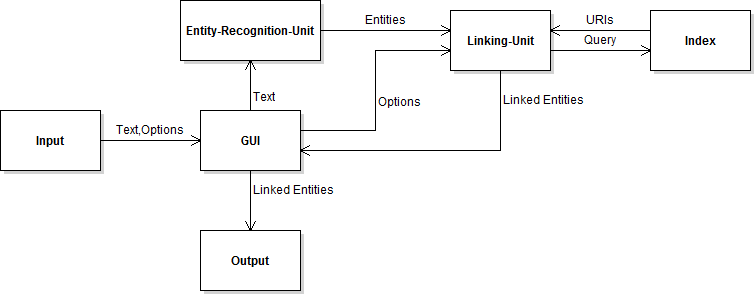
\includegraphics[scale=0.55]{./system.png}
\caption[System\"ubersicht]{System\"ubersicht}
\end{figure}


\section{Graphical User Interface}
Die GUI stellt die Schnittstelle zwischen Benutzer und Programm dar. Diese erlaubt ihm, seinen zu anotierenden Text zu \"ubergeben und zwischen verschiedenen Optionen zu w\"ahlen. Der Input wird entgegenommen und dessen Text an die Entity-Recognition-Unit weitergeleitet. Am Ende bekommt es die verlinkten Entities von der Linking-Unit zur\"urck und gibt diese an den Benutzer weiter.
\begin{figure}[!ht]
\centering
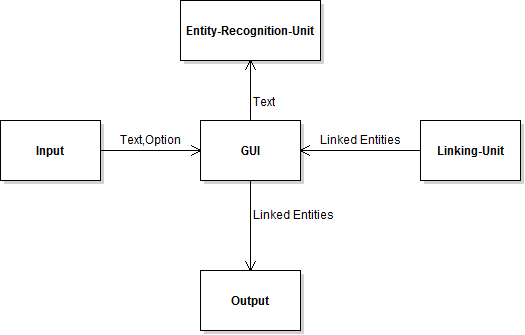
\includegraphics[scale=0.55]{./GUI.png}
\caption[GUI]{GUI-Verbindungen}
\end{figure}


\section{Enitity-Recogniction-Unit}
Diese Einheit ist f\"ur die Erkennung von Named Entities verantwortlich. Dies bedeutet, dass sie den ihr \"ubergebenen Text analysiert und alle sich darin befindlichen Entit\"aten extrahiert (z.B. Personen oder Orte). Das Ergebnis dieses Prozesses wird dann an die Linking-Unit weitergeleitet.
\begin{figure}[ht!]
\centering
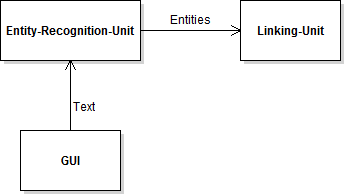
\includegraphics[scale=0.55]{./eeu.png}
\caption[EEnitity-Recognition-Unit]{Enitity-Recognition-Unit}
\end{figure}


\section{Linking-Unit und Index}
Die Linking-Unit versucht mit Hilfe des Indexes f\"ur jede an sie weitergeleitete Entit\"at einen passenden uniform resource Identifier (URI) zu finden. Dazu erstellt sie, unter Ber\"ucksichtigung der vom Benutzer eingestellten Optionen, eine Query und l\"asst den Index diese ausf\"uhren. Dessen R\"uckgabewert wird dann mit den Named Entities verkn\"upft und an die GUI weitergereicht.
\begin{figure}[ht!]
\centering
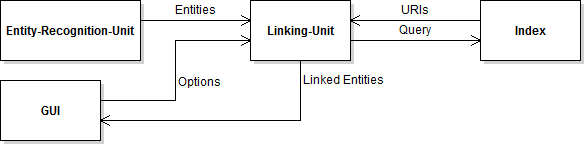
\includegraphics[scale=0.55]{./linking.png}
\caption[Linking Unit]{Linking-Unit}
\end{figure}
\section{Informationsfluss}
Um die Informationsverarbeitung noch einmal in einer Gesamt\"ubersicht zu betrachten, sind alle Abl\"aufe in dem folgenden Sequenzdiagramm verdeutlicht.
Folgende Szenarien sind abgedeckt :
\begin{itemize}
\item Texteingabe
\item Optionsauswahl
\item Annotierung
\end{itemize}

\begin{figure}[ht!]
\centering
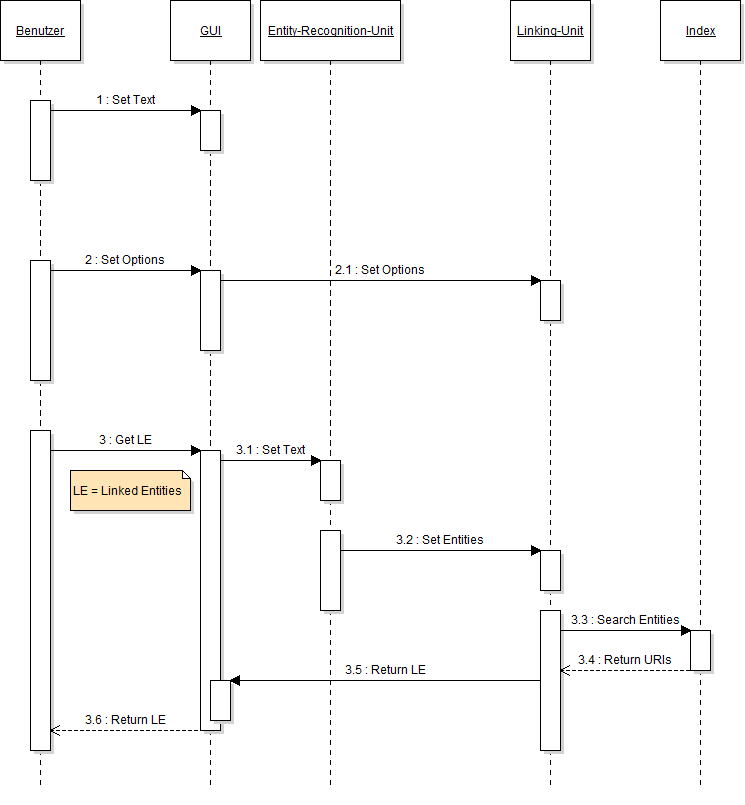
\includegraphics[scale=0.55]{./seq.png}
\caption[Programmablauf]{Programmablauf}
\end{figure}
%----------------------------------------------------------------------------
\chapter{Implementierung}
\label{Kapitel 3}
\lhead{Kapitel 3.}
\chead{\emph{Implementierung}}
Der Source-Code f\"ur den Index Based Entity Linker(IBEL) wird als ein  Maven\footnote{\url{http://maven.apache.org/}}-Projekt f\"ur Java verwaltet. Dies erm\"oglicht ein komfortables Warten und Weiterentwickeln des Codes, da alle ben\"otigten Bibliotheken automatisch \"uber das zentrale Maven-Repository bezogen werden. Zus\"atzlich ist sichergestellt, dass diese die richtige Version besitzen, um Kompatibilitätsprobleme zu vermeiden.\\
Als Entwicklungsumgebung wurde Netbeans 8.0 verwendet und als Java-Version Java 7. 
Im Folgenden wird nun die Implementierung der einzelnen Funktions-Einheiten, welche in Kapitel \ref{Kapitel 2} vorgestellt wurden, behandelt.

\section{GUI und Controller}
Um die einzelnen Bestandteile des IBEL zu kapseln und somit leichter zu Warten, wurde eine Controller implementiert, dessen alleinige Aufgabe es ist, die Kommunikation zwischen den Klassen zu handhaben. \\
Die Gui nimmt weiterhin die Eingaben des Benutzers entgegen, jedoch wird die Auswertung der Interaktion nun von dem Controller \"ubernommen. Hierf\"ur implementiert dieser das ActionListener-Interface des java.awt.event-Packages.
\begin{figure}[ht!]
\centering
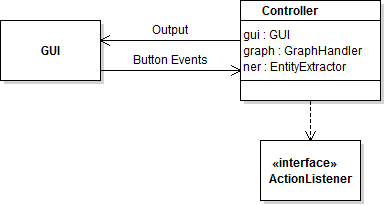
\includegraphics[scale=0.55]{./guiCont.png}
\caption[GUI and Controller]{GUI and Controller}
\end{figure}

\section{Enitity-Recognition-Unit}
\label{Kapitel 3.2}
Um den vom Benutzer eingegeben Text untersuchen zu k\"onnen, benutzt IBEL den Stanford-NER, einen von der Universit\"at Stanford entwickelten Named Entity Recognizer, der Wortsequenzen in einem Text kennzeichnet, bei denen es sich um Namen f\"ur Dinge handelt, wie zum Beispiel Personen oder Firmennamen \footnote{\url{http://nlp.stanford.edu/software/CRF-NER.shtml}}. 
\begin{figure}[ht!]
\centering
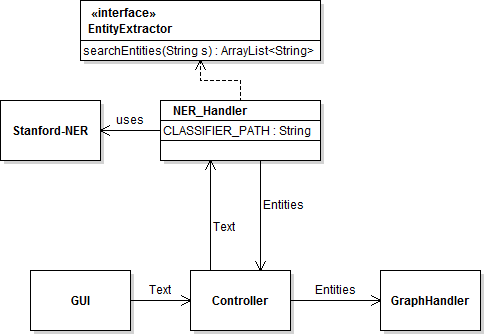
\includegraphics[scale=0.55]{./eruImp.png}
\caption[Entity-Recognition-Unit Impl.]{Entity-Recognition-Unit Implementation}
\end{figure}

Die Schnittstelle zwischen dem Controller und der Enitity-Recognition-Unit (ERU) bildet das EntityExtractor-Interface. Jede Klasse, die dieses implementiert, kann vom Controller genutzt werden, um Entit\"aten in Texten erkennen zu lassen. Der NER\_Handler, welcher dieses Interface implementiert, nutzt die Classifier des Stanford-NER, um eine Liste mit Entit\"aten in dem ihm \"ubergebenen Text zu extrahieren.

\section{Linking-Unit}
Nachdem die Entity-Recognition-Unit alle gefundenen Entit\"aten an den Controller\\ zurückgeben hat, werden diese an den GraphHandler zum Entity Linking weitergeleitet. Dieser erstellt Querys f\"ur Lucene, einer performanten Open Source Java-Bibliothek f\"ur Textsuche\footnote{\url{http://lucene.apache.org/core/}}, und l\"asst diese dann ausf\"uhren. Die ermittelten URIs werden mit den Entit\"aten verkn\"upft und an den Controller zur\"uckgegeben.
\begin{figure}[ht!]
\centering
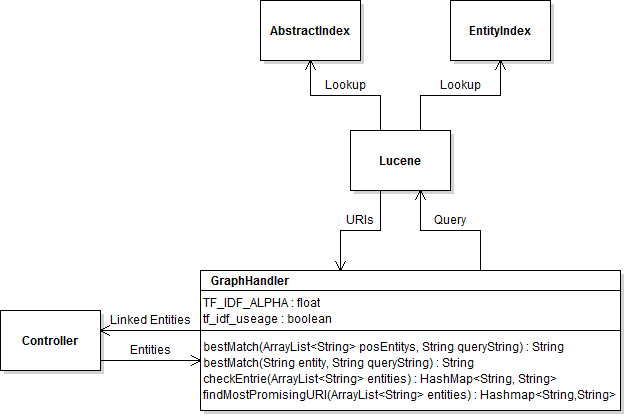
\includegraphics[scale=0.55]{./entLinkImp.png}
\caption[Entity Linking Unit]{Entity Linking Unit}
\end{figure}

\subsection*{Ablauf des Linkings}

Der Entity-Linking-Algorithmus erh\"alt eine Liste von Entit\"aten und durchl\"auft dann drei Phasen:
\begin{enumerate}
\item Titelvergleich: Es wird geschaut, ob die Entit\"at ein Titel f\"ur eine DBpedia Seite ist. Zum Beispiel w\"are die Entit\"at \glqq United States\grqq{} der Titel der DBpedia Seite mit der URI \glqq http://dbpedia.org/resource/United\_States\grqq{} .

\item Anchorsuche: Falls die Titelsuche kein Ergebnis liefert, so wird \"uberpr\"uft, ob die Entit\"at ein verzeichneter Anchor einer URI ist. In dem United States Beispiel w\"are \glqq USA\grqq{} einer dieser Anchors. Da ein Anchor disambig sein kann, wird versucht, \"uber den semantischen Kontext eine Entscheidung zu treffen. Dazu werden die Nachbaranchors der möglichen Kandidaten mit allen anderen gefunden Entit\"aten verglichen. Der Kandidat mit den meisten \"Ubereinstimmungen hat die grö\ss te Wahrscheinlichkeit, die gesuchte URI zu sein und wird deshalb mit der Entit\"at verkn\"upft.

\item tf-idf-Suche: Wurde in den ersten beiden Schritten keine passende URI gefunden und der Benutzer hat die entsprechende Option angegeben, so wird versucht \"uber eine tf-idf-Suche eine URI zu ermitteln. Dazu wird in den Abstract-Texten aller DBpedia Seiten nach dem Vorkommen der Entit\"at gesucht. Der \grqq term frequencey\grqq{}-Wert (tf) gibt dabei an, wie h\"aufig die Entit\"at gefunden wurde und die \grqq inverse document frequencey\grqq{} (idf) wertet die Bedeutung im Kontext mit allen Dokumenten (in diesem Falle DBpedia Seiten). Die 20 erfolgreichsten Suchtreffer werden nun behandelt als w\"aren sie Kandidaten f\"ur einen disambiguen Anchor. Mit ihnen wird wie in der vorherigen Phase verfahren.
\end{enumerate}

Pseudocode :
\begin{lstlisting}
function findURIs(List entities)
	map<k,v> result;
	URI tmp;
	forall entity in entities
		tmp=searchTitle(entity)				\\titelsuche
		if(tmp!=null)
			result.put(entity,tmp);
		else
			tmp=anchorSearch(entity)		\\Anchorsuche
			if(tmp!=null)
				result.put(entity,tmp);
			else if(tf_idf_Search==true)
				list posURIs=tf_idf_Lookup(entity)\\Abstractsuche
				tmp=anchorSearch(posURIs)\\Anchorsuche mit 
							\\Abstractsuchergebnissen
				result.put(entity,tmp)
			endif
		endif
	endfor
	return result;
\end{lstlisting}
\clearpage
In dem Folgenden Aktivit\"atsdiagramm wird noch einmal der Linking-Algorithmus verdeutlicht.
\begin{figure}[ht!]
\centering
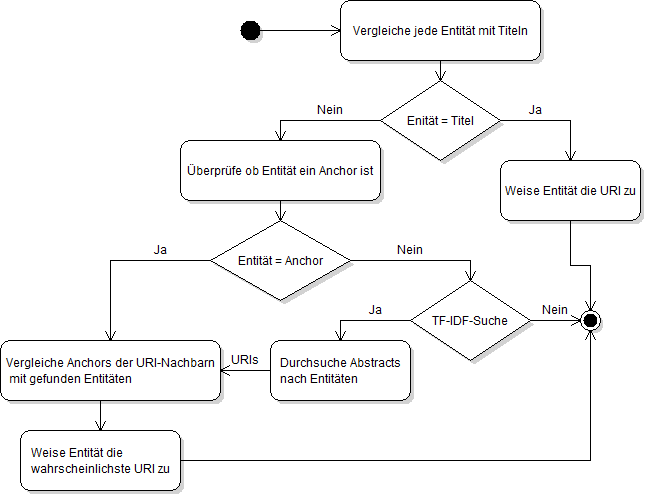
\includegraphics[scale=0.55]{./ablauf.png}
\caption[Entity Linking]{Entity Linking}
\end{figure}


\section{Index}
%\footnote{\url{http://lucene.apache.org/core/4_6_0/join/org/apache/lucene/search/join/ToParentBlockJoinQuery.html}}
Ein Lucene-Index ist eine indexierte Ansammlung von Dokumenten. Ein Dokument besitzt eine beliebige Anzahl von Feldern, in denen Informationen gespeichert werden k\"onnen. 
Der Index aus der System\"ubersicht wurde in der Implementierung in 2 Indexe unterteilt. Dies liegt haupts\"achlich daran, dass sie unterschiedliche Formate  besitzen, um die aufgabenspezifischen Querys effizienter zu machen.
\subsection{EntityIndex}
Der EntityIndex wurde als BlockIndex angelegt, d.h. er besitzt zwei unterschiedliche Dokumenttypen:
\begin{enumerate}
\item Kinddokument: Ein Kinddokument ist ein gew\"ohnliches Dokument.
\item Elterndokument: Elterndokumente unterscheiden sich von Kinddokumenten durch ein Indikatorfeld, das f\"ur alle Elterndokumente den gleichen Wert hat.
\end{enumerate}
Um Eltern und deren Kinder bei der Queryauswertung richtig zuordnen zu k\"onnen, muss bei der Indexerstellung eine bestimmte Reihenfolge eingehalten werden: Erst werden alle Kinddokumente eines gleichen Elter hinzugef\"ugt, gefolgt von dem Elterndokument.\\
Dieses besondere Format erm\"oglicht \texttt{ToParentBlockJoinQuerys}. Diese Querys selektieren erst Elterndokumente und f\"uhren dann eine weitere Query auf den Kindern dieser Eltern aus. Dadurch kann sehr gezielt und somit effizient gesucht werden.\\
In der Implementation repr\"asentieren Elterndokumente die einzelnen Seiten aus DBpedia. Sie speichern den Titel, die URI und alle Anchors einer Seite. Die Kinddokumente  besitzen nur ein Feld mit einem Anchor eines Nachbarn der URI aus dem Elterndokument.\\
Zur Veranschaulichung wird hier noch einmal das Format des EntityIndexes gezeigt:
\begin{lstlisting}
<anchorN$_{1_1}$> (Kind 1 von URI$_1$)
...
<anchorN$_{n_1}$> (Kind n von URI$_1$)
<URI$_1$,anchor$_{1_1}$ ... anchor$_{i_1}$,title$_1$,type> (Elter der Kinder 1 - n) 
\end{lstlisting}
\subsection{AbstractIndex}
Der AbstractIndex ist ein Standart-Index, dessen Dokumente zwei Felder enthalten:
\begin{enumerate}
\item URI
\item Abstract der URI
\end{enumerate}
Sein Format sieht wie Folgt aus:
\begin{lstlisting}
<URI$_1$,abstract$_1$>
...
<URI$_n$,abstract$_n$>
\end{lstlisting}
Da Lucene f\"ur sein Query-Scoring tf-idf-Werte verwendet und auch genau diese bei der Abstract Suche erw\"unscht sind, liefert eine normale Query bereits das gew\"unschte Ergebnis.
%------------------------------------------------------------------------
\chapter{Evaluierung}
\label{Kapitel 4}
\lhead{Kapitel 4.}
\chead{\emph{Evalurierung}}

Dieses Kapitel besch\"aftigt sich intensiv mit der Analyse des Linking-Algorithmus. Insbesondere wird auf die Aspekte Geschwindigkeit und Genauigkeit eingegangen. Als Basis f\"ur die Auswertung wurden Texte aus Wikipedia\footnote{\url{www.wikipedia.org}} genommen und f\"ur die Semantik-Analyse Datens\"atze des Max Plank Institutes.\\
Die Tabellen f\"ur die Graphen finden sich im Anhang.

\section{Geschwindigkeit}
Der ma\ss geblichste Faktor der Geschwindigkeit ist die Benutzungsdauer des Programms. Man spricht hierbei von einem "warmed up Index", was bedeutet, dass aufgrund von Cashe-Eintr\"agen Daten schneller ermittelt werden k\"onnen.
\subsection{Unwarmed Mode}
Da der \grqq warmed up\grqq{}-Modus sehr inkonsistente Ergebnisse f\"ur wiederholte Versuche mit gleichen Texten liefert, wird der \grqq unwarmed mode\grqq{} betrachtet, in dem das Programm noch \"uber keinerlei Cashe-Eintr\"age f\"ur Querys verf\"ugt. Dies ist auch gleichzeitig eines der Worst-Case-Szenarien des Linking-Algorithmus.\clearpage
In einem durchschnittlichen Text lassen sich fast 80\% aller , durch den Stanford-NER, gefundenen Entit\"aten entweder mit einem Titel oder einem Anchor verbinden. Der Rest muss mit Hilfe von tf\_idf-Werten bestimmt werden.
\begin{figure}[ht!]
\centering
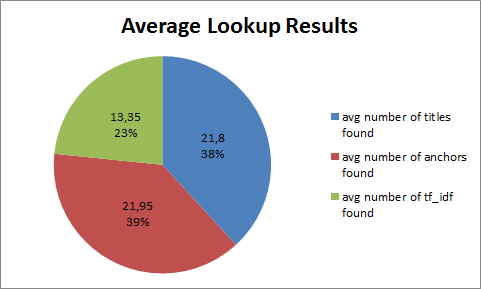
\includegraphics[scale=1]{./lookupRes.png}
\caption[Average Lookup Results]{Average Lookup Results}
\end{figure}

Um die einzelnen Operationen in einem zeitlichen Zusammenhang betrachten zu k\"onnen, wird als n\"achstes die durchschnittlich ben\"otigte Zeit f\"ur jede dieser Operationen betrachtet. 
\begin{figure}[ht!]
\centering
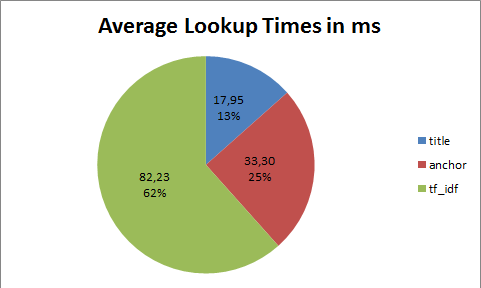
\includegraphics[scale=1]{./lookupTime.png}
\caption[Average Lookup Times]{Average Lookup Times}
\end{figure}

Wie man in der Abbildung gut sehen kann, sind Titel- und Anchorsuche g\"unstige Operationen im Vergleich zu der tf-idf-Suche, wobei die Titelsuche fast doppelt so schnell ver\"auft wie die Anchorsuche. Im Idealfall sollten die zu linkenden Entit\"aten entweder ein Titel oder ein Anchor sein.

\textbf{Anmerkung}: Bei der Abbildung handelt es sich nur um die ben\"otigte Zeit der verschiedenen Operationen. Da diese aber sequentiell ablaufen, bedeutet dies, dass die Linking-Zeit der Summe der benutzten Operationen entspricht (z.B. betr\"agt die Zeit f\"ur Anchor-Linking Titel-Lookup + Anchor-Lookup).
\subsection{Warmed Up}
Zum Vergleich mit einem \grqq warmed up Index \grqq{} wurde eine H\"alfte der Testtexte benutzt, um Cashe-Eintr\"age anzulegen, und die andere H\"alfte wurde  normal annotiert. Das Ergebnis ist ein deutlicher Anstieg in Geschwindigkeit.
\begin{figure}[ht!]
\centering
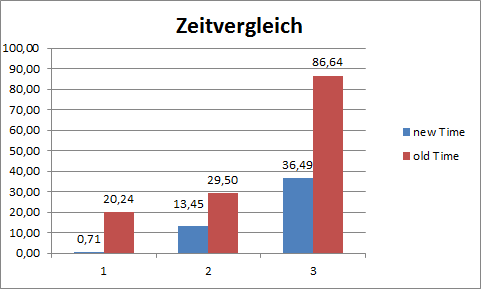
\includegraphics[scale=1]{./zeitvergleich.png}
\caption[Zeitvergleich warmed vs unarmed]{Zeitvergleich}
\end{figure}

Um diesen Effekt zu maximieren, sollten thematisch verwandte Texte sequentiell annotiert werden.


\section{Genauigkeit}
Nach der Betrachtung der Geschwindigkeit ist nun die Ergebnis-Qualit\"at der einzelnen Operationen interessant. Dazu wurden die Ergebnisse des IBEL mit den Ergebnissen von DBpedia Spotlight vergleichen.
\subsection{Titelsuche}
Da die Titelsuche nur f\"ur exakte \"Ubereinstimmungen ein Ergebnis liefert, werden die Entit\"aten nahezu immer richtig verlinkt. Eine Fehlverlinkung tritt nur auf, wenn eine Entit\"at mit einem Titel \"ubereinstimmt, aber dieser im semantischen Kontext eine andere Bedeutung hat.\\
\textbf{Beispiel}:\\
Tiger was lost in the woods when he got divorced from Elin.\footnote{Auszug des KORE50-Datensatzes des Max Planck Instituts} \\Der Stanford-NER liefert f\"ur diesen Satz die zwei Entit\"aten Tiger und Elin zur\"uck. Die Titelsuche findet dann f\"ur Tiger die URI \texttt{http://dbpedia.org/resource/Tiger}. Richtig w\"are in diesem Falle aber \texttt{http://dbpedia.org/resource/Tiger\_Woods}.

\subsection{Anchorsuche}
Die Anchorsuche besitzt die selben Eigenschaften wie die Titelsuche. Ihre Ergebnisse sind sehr Pr\"aziese und nur falsch, wenn durch den semantische Kontext eine andere Bedeutung entsteht.

\textbf{Anmerkung}: Jeder Titel einer DBpedia-Seite ist auch gleichzeitig ein einzigartiger Anchor. Dies bedeutet das die Titelsuche ebenfalls eine Anchorsuche ist, aber nur auf der Menge der eindeutigen Anchors. W\"urde die Titelsuche deaktiviert werden, so w\"urde IBEL trotzdem das gleiche Ergebnis zur\"uck liefern, aber mehr Zeit in Anspruch nehmen.   

\subsection{Tf-Idf-Suche}
Die tf-idf-Suche ist im Vergleich zu den ersten beiden Suchenmethoden sehr unzuverl\"assig. Sie ermittelt zwar eine URI f\"ur eine Seite, die zu dem   semantischen Kontext und der Entit\"at passt, ist aber meistens eine falsche Verlinkung. Folgende Ursachen k\"onnen daf\"ur verantwortlich sein:
\begin{itemize}
\item Die Entit\"at besitzt keine passende DBpedia-Seite.
\item Der indexierte Abstract-Text der richtigen DBpedia-Seite ist zu kurz um eine Disambiguirung zu erm\"oglichen.
\item Eine thematisch nahe verwandte DBpedia-Seite besitzt einen gr\"o\ss eren Abstract-Text mit mehr Referenzen auf die Entit\"at.
\item Der Stanford-NER hat ein falsches Ergebnis geliefert.
\end{itemize}
Der letzte Fall ist besonders von Interesse, da die tf-idf-Suche eine sehr teure, optionale Operation ist. Bei der Verlinkung der Test-Texte wurde diese Suche f\"ur 220 Kandidaten verwendet. Circa 56\% davon waren falsche Entit\"aten, wie zum Beispiel die Adjektive german, russian und jewish .
\begin{figure}[ht!]
\centering
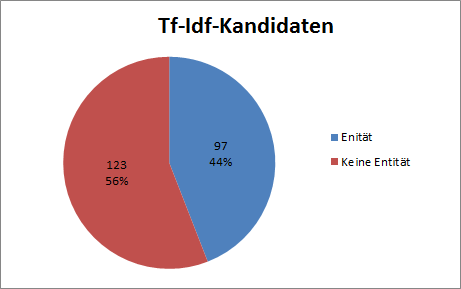
\includegraphics[scale=1]{./tfPrecision.png}
\caption[Tf-Idf-Kandidaten]{Tf-Idf-Kandidaten}
\end{figure}

\section{Semantikanalyse mit KORE}
Das Max Planck Institut f\"ur Informatik\footnote{\url{http://www.mpi-inf.mpg.de/index\_d.php}} bietet von Hand gefertigte Datens\"atze zum Testen von Disambiguirungsalgorithmen. Diese Keyphrase Overlap Relatedness for Entity Dismabiguation (KORE)\footnote{\url{http://www.mpi-inf.mpg.de/yago-naga/aida/download/KORE50.tar.gz}} Testdaten sind so erstellt, dass sie besonders schwer zu disambiguieren sind. \\
Da nahezu alle vom Stanford-NER erkannten Entit\"aten in diesen Texten ihre Bedeutung nur \"uber den semantischen Kontext erhalten und dies genau die Schw\"ache der Titel- und Anchorsuche sind, schneidet der Index Based Entity Linker (IBEL) schlecht ab. 
\begin{center}
\begin{tabular}{|l|l|l|l|l|}
\hline
Ent\"aten ges. & Ent\"aten gefunden & Anchors erkannt & richtig Verlinkt  \\
\hline
148 & 130 (87,8 \%) & 75 (50,6 \%) & 26 (17,6 \%) \\
\hline
\end{tabular}
\end{center}

Insgesamt wurden also nur 17,6\% aller Entit\"aten richtig verlinkt. Zwar k\"onnen  \"uber 50\% mit einem Anchor verbunden werden, aber viele dieser Anchors sind eindeutig und bieten somit keine M\"oglichkeit zur semantischen Interpretation.\\
\textbf{Beispiel}:\\
David and Victoria added spice to their marriage.\footnote{Auszug des KORE50-Datensatzes des Max Planck Instituts} \\
Gesucht werden die Entit\"aten David und Victoria Beckham. Diese besitzen aber nur Variationen der Schreibweise ihrer vollen Namen (z.B. David Beckam, David Beckham und David\_Beckham) oder Dinge, die sie identifizieren (z.B Posh Spice, ein Album von Victoria Beckham) als Anchor, jedoch nicht David oder Victoria. Diese beiden sind n\"amlich f\"ur die URIs \texttt{http://dbpedia.org/resource/David} und \\ \texttt{http://dbpedia.org/resource/Victoria} eindeutig.

Dies f\"uhrt dazu, dass viele Entit\"aten falsch verlinkt werden.
\clearpage
\section{Vergleich mit DBpedia}
Der Index Based Entity Linker (IBEL) liefert f\"ur alle getesteten Texte \"ahnlich gute Ergebnisse. Jedoch ist DBpedia Spotlight IBEL im Bezug auf Semantikanalyse noch \"uberlegen.

\begin{center}
\begin{tabular}{|l|l|l|l|l|}
\hline
Ent\"aten ges. & Ent\"aten gefunden & richtig Verlinkt  \\
\hline
148 & 46 (31 \%) & 30 (20,3 \%) \\
\hline
\end{tabular}
\end{center}

Zwar schneidet DBpedia Spotlight mit 20\% richtig verlinkten Entit\"aten ebenfalls nicht gut bei den KORE-Datens\"atzen ab, aber etwas besser als IBEL.
Beide Programme haben also \"ahnliche Schw\"achen.


%-------------------------------------------------------------------------
\chapter{Deployment und Erweiterung auf andere Sprachen}
\label{Kapitel 5} % Change X to a consecutive number; for referencing this chapter elsewhere, use \ref{ChapterX}

\lhead{Kapitel 5.}
\chead{\emph{Deployment und Erweiterung auf andere Sprachen}}
\section{Deployment}
Um das Programm zu deployen muss lediglich die JAR mit compilierten Dependencies(falls das Programm aus dem Sourcecode compiliert wurde, ist dies die \\\grqq IndexBasedEntityLinker-1.0-jar-with-dependencies.jar\grqq), sowie ein passender Entity- und Abstract-Index in ein gleiches Verzeichnis kopiert werden.
\subsection{Generierung der Indexe mit Utility-1.0}
Sollten keine gültigen Indexe vorhanden sein, so k\"onnen diese entweder manuell oder \"uber die IndexBasedEntityLinker\_Utility(IBELU) generiert werden.
\begin{figure}[ht]
\centering
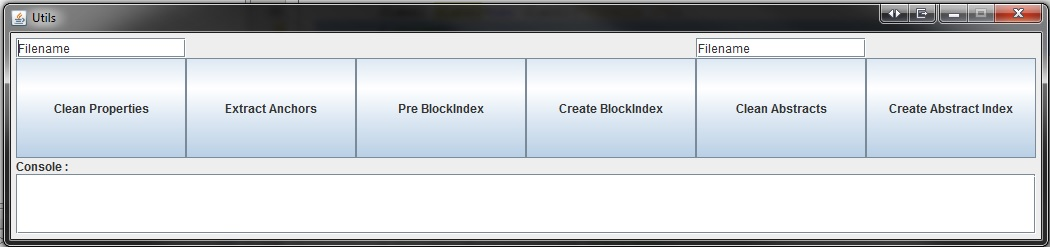
\includegraphics[scale=0.52]{util.jpg}
\caption[Index Based Entity Linker Utility]{Index Based Entity Linker Utility}
\end{figure}
\clearpage
Daf\"ur werden folgende Dateien ben\"otigt:
\begin{itemize}
\item Der DBpedia Anchor-Index der Computer Semantic Group der Universit\"at Bielefeld
\item Mapping-based Properties (en) von DBpedia\footnote{\url{http://downloads.dbpedia.org/3.9/en/mappingbased\_properties\_en.nt.bz2}}
\item Extended Abstracts (en) von DBpedia\footnote{\url{http://downloads.dbpedia.org/3.9/en/long\_abstracts\_en.nt.bz2}}
\end{itemize}
Die Abfolge der auszf\"uhrenden Operationen ist von links nach rechts sortiert und sollte auch in dieser Reihenfolge abgewickelt werden.\\
Zur Erstellung des Entity-Indexes werden der Anchor-Index und die Mapping-based Properties ben\"otigt. Der Ablauf ist wie folgt:
\begin{enumerate}
\item Clean Properties: In dem zugeh\"origen Textfeld oberhalb des Buttons muss der Dateipfad (lokal oder absolut) zu der Mapping-Based Properties Datei angegeben werden. Diese wird dann von allen irrelevanten Daten ges\"aubert.\\
Output: cleaned\_properties.txt, cleaned\_properties\_neigborToEntity.txt und \\entities.txt.
\item Extract Anchors: Liest den Anchor-Index aus und schreibt alle \\ \textless URI,anchor\textgreater-Paare in eine Datei.\\
Output: anchors.txt
\item Pre BlockIndex: Erstellt f\"ur die Schnittmenge der URIs aus entities.txt und anchors.txt Dateien zur BlockIndex Generierung.\\
Output:combined.txt, entity\_anchors.txt, entity\_neighbor\_anchorsN.txt,
\\neighbor\_entity\_anchorsE.txt
\item Create BlockIndex Erzeugt den BlockIndex(EntityIndex).\\
Output : Blockindex
\end{enumerate}

Zu Generierung des Abstract-Indexes werden die entities.txt aus dem ersten Teil und die Long-Abstracts ben\"otigt:
\begin{enumerate}
\item Clean Abstracts: Nach Angabe des Dateipfades (lokal oder absolut) der\\ long-abstracts-Datei werden f\"ur alle URIs die ein Abstract besitzen und in entities.txt vorkommen \textless URI, abstract\textgreater-Paare erstellt und gespeichert.\\
Output: abstract\_clean.txt
\item Create Abstract Index: Erstellt den Abstract-Index.\\
Output:Abstract Index
\end{enumerate}
\"Uber Erfolg oder Misserfolg (Fehlermeldungen) der ausgef\"uhrten Operationen wird der Benutzer der IBELU \"uber ein Konsolen-Feld (siehe Abbildung 5.1) informiert.

\textbf{Anmerkung}: Diese Operationen sind teilweise sehr speicherintensiv. Es sollten mindestens 12GB RAM zur Verf\"ugung gestellt werden und sichergestellt sein, dass die JVM diesen auch nutzen darf (VM Parameter: -Xmx12g).


\subsection{Eigenst\"andige Generierung von Dateien}
Die IBELU kann auch nur zur reinen Indexerstellung genutzt werden, w\"ahrend die daf\"ur ben\"otigten Dateien anderweitig erstellt werden. Im Nachfolgenden werden die Dateien und ihre Formate n\"aher erl\"autert.
\subsubsection*{Dateien zur Erstellung des Entity-Indexes}
Um den Index \"uber die IBELU zu erstellen, sind zwei Dateien erforderlich:
\begin{itemize}
\item combined.txt: In dieser Datei werden alle URIs auf ihre Nachbarn und deren Anchors gemappt. Ein Nachbar einer URI A ist in diesem Fall eine URI B, deren Graphknoten eine Kante zu dem Knoten von A besitzt.\\
Format:
\begin{lstlisting}
URI$_1$|Neighbor$_1$|anchor$_{1,1}$;...;anchor$_{1,i}$
...
URI$_1$|Neighbor$_{m_1}$|anchor$_{m_1,1}$;...;anchor$_{m_1,j}$
...
...
URI$_n$|Neighbor$_{m_n}$|anchor$_{m_n,1}$;...;anchor$_{m_n,k}$
\end{lstlisting}
\item entity\_anchors.txt: Diese Datei mappt alle URIs auf ihre Anchors.\\
Format:
\begin{lstlisting}
URI$_1$|anchor$_{1,1}$;...;anchor$_{1,i}$
...
...
...
URI$_n$|anchor$_{n,1}$;...;anchor$_{n,j}$
\end{lstlisting} 
\end{itemize}
Diese Dateien sollten lexikographisch sortiert sein, um den resultierenden Index performanter zu machen.

\textbf{Anmerkung}: Nat\"urlich k\"onnen auch die Indexe eigenst\"andig erstellt werden. Aufbau und Funktionsweise werden in dem Kapitel \glqq Implementierung \grqq ausf\"uhrlich behandelt.
\section{Erweiterung um andere Sprachen}
Um IBEL mit anderen Sprachen nutzen zu k\"onnen, m\"ussen neue Indexe erstellt und die existierende Entity-Recognition-Unit angepasst beziehungsweise ersetzt werden.

\subsection{Indexe}
F\"ur jede zu unterst\"uzende Sprache muss ein neuer Entity-Index und ein neuer Abstract-Index erstellt werden. In Kapitel 5.1 wurde dies bereits ausf\"uhrlich behandelt.
Die daf\"ur ben\"otigten Mapping-Based Properties sowie die long-Abstracts werden von DBpedia in 119 verschieden Sprachen zur Verf\"ugung gestellt. \\
Die entsprechenden Anchors f\"ur diese Sprache müssen allerdings entweder eigenst\"andig generiert oder aus einer anderweitigen Quelle bezogen werden.
\clearpage
\subsection{Entity Recognition}
F\"ur die Entity-Recognition-Unit kann, durch einen Austausch der Klassifizierer, weiterhin der Stanford-NER verwendet werden.  
Auf der Downloadseite des Stanford-NER\footnote{\url{http://nlp.stanford.edu/software/CRF-NER.shtml}} finden sich Klassifizierer f\"ur die deutsche und chinesische Sprache. F\"ur andere Sprachen m\"ussen eigene Klassifzierer trainiert werden. Das n\"otige Vorgehen daf\"ur ist auf der FAQ-Seite\footnote{\url{http://nlp.stanford.edu/software/crf-faq.shtml\#a}} beschrieben. Um den neuen Klassifizierer nutzen zu k\"onnen, muss der Ladepfad in der CLASSIFIER\_PATH-Variable in der Klasse NER-Handler entsprechend angepasst werden.

Es wird auch jede andere Implementation von Named-Entity-Regocnition unterst\"utz. Daf\"ur muss lediglich ein  Adapter\footnote{\url{http://de.wikipedia.org/wiki/Adapter
\_(Entwurfsmuster)}} geschrieben werden, welcher das EntityExtractor-Interface implementiert. Dieser muss dann in der Klasse App.java der GUI anstelle des NER\_Handlers im Konsturktoraufruf \"ubergeben werden.

\textbf{Anmerkung}: Da das Programm im Nachhinein in eine Serverapplikation f\"ur die Semantic Computer Group umgebaut wird, wird die GUI voraussichtlich nicht mehr verwendet werden. Daher muss der Adapter dann den NER\_Hanlder an einer anderen Stelle ersetzen.

\chapter{Zusammenfassung und Ausblick}
Zusammenfassend kann man sagen, dass der Index Based Entity Linker (IBEL) eine gute Alternative zu DBpedia Spotlight ist, aber in einigen F\"allen noch ein wenig unpr\"azieser. Insgesamt ist es ein Programm, das schnell und zuverl\"assig Enitit\"aten, die einen Anchor besitzen und durch den semantischen Kontext keine andere Bedeutung erhalten, annotieren kann. Wenn man thematisch verwandte Texte sequentiell annotiert, ist sogar ein deutlicher Anstieg in der Geschwindigkeit messbar, da IBEL \"uber Cache-Eintr\"age Daten schnell erneut Abrufen kann. \\
Im Bereich der fortgeschrittenen Semantikanalyse, wie sie die KORE-Datens\"atze fordern, besteht noch Verbesserungsbedarf, da die tf-idf-Suche noch sehr ungenau ist und eindeutige Anchors keinen Raum f\"ur semantische Interpretation lassen, obwohl es f\"ur diese Texte notwendig w\"are. IBEL bietet an diesen Stellen noch viel Platz f\"ur Optimierung und Erweiterung. Unter anderem k\"onnen folgende Vorschl\"age zur Verbesserung getestet werden :
\begin{itemize}
\item L\"angere und ausf\"uhrlichere Abstract-Texte.
\item Wenn f\"ur eine Entit\"at kein Titel oder Anchor gefunden wird, anstelle der tf-idf-Suche einen \"Ahnlichkeitsabgleich mit anderen Anchors machen (bei der Anchor-Suche wird derzeit nur ein exakter Treffer verwendet) und dann eine.
\item die tf-idf-Querygewichte in Abh\"anigkeit zu dem tf-idf-score dynamisch anpassen.
\item Kombinationen der vorherigen Punkte.
\end{itemize}
Weiterhin sollte der Stanford-NER eventuell gegen einen anderen Name and Entity Recognitioner ausgetauscht werden, da dieser noch fehlerhafte Ergebnisse, wie zum Beispiel Adjektive, zur\"uckliefert. Durch den modularen Aufbau von IBEL ist ein solcher Austausch\footnote{siehe Kapitel \ref{Kapitel 3.2}} sehr einfach zu realisieren.\\
Schlussendlich kann der Index Based Entity Linker, wie in Kapitel \ref{Kapitel 5} beschrieben, um weitere Sprachen erweitert werden. Daf\"ur werden lediglich zwei zus\"atzliche Indexe pro Sprache und eine Option zum Umschalten zwischen den Indexen ben\"otigt.




%----------------------------------------------------------------------------------------
%	THESIS CONTENT - APPENDICES
%----------------------------------------------------------------------------------------

\addtocontents{toc}{\vspace{2em}} % Add a gap in the Contents, for aesthetics

\appendix % Cue to tell LaTeX that the following 'chapters' are Appendices
\chapter{Evaluierungstabellen}

\begin{figure}[!ht]

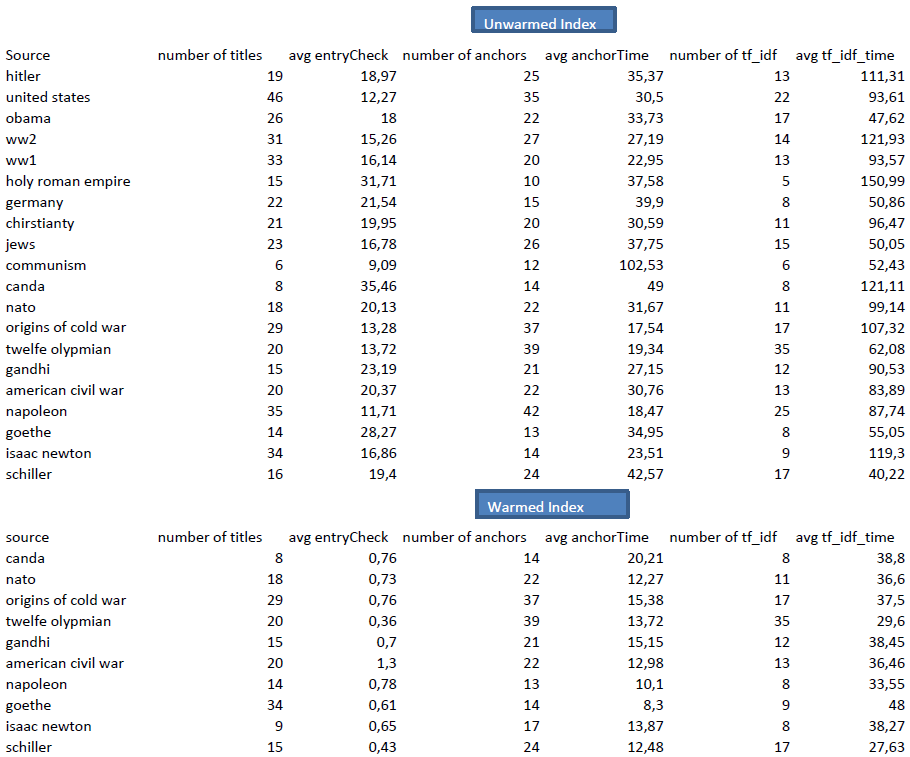
\includegraphics[scale=0.65,angle=270]{eval.png}
\end{figure}

% Include the appendices of the thesis as separate files from the Appendices folder
% Uncomment the lines as you write the Appendices




\addtocontents{toc} % Add a gap in the Contents, for aesthetics

\backmatter

%----------------------------------------------------------------------------------------
%	BIBLIOGRAPHY
%----------------------------------------------------------------------------------------

\label{Quellen}

\lhead{\emph{Quellen}} % Change the page header to say "Bibliography"

\bibliographystyle{alpha} % Use the "unsrtnat" BibTeX style for formatting the Bibliography
%\nocite{*}


\bibliography{Bibliography}
\section*{Internetquellen}
\begin{itemize}
\item \url{http://maven.apache.org/}
\item \url{http://nlp.stanford.edu/software/CRF-NER.shtml}
\item \url{http://lucene.apache.org/core/}
\item \url{www.wikipedia.org}
\item \url{http://www.mpi-inf.mpg.de/index\_d.php}
\item \url{http://www.mpi-inf.mpg.de/yago-naga/aida/download/KORE50.tar.gz}
\item \url{http://de.wikipedia.org/wiki/Adapter
\_(Entwurfsmuster)}
\item \url{http://nlp.stanford.edu/software/crf-faq.shtml\#a}
\item \url{dbpedia.org}
\item \url{http://www.w3.org/DesignIssues/LinkedData.html}
\item \url{spotlight.dbpedia.org}
\item \url{http://webknox.com/p/linked-open-data-visualization}
\item \url{http://www.sc.cit-ec.uni-bielefeld.de/}
\end{itemize}
\end{document}  